\documentclass[14pt]{extreport}
\usepackage{gost}

%Тут можно вставить дополнительные пакеты

\begin{document}
\pagestyle{empty} %  выключаем нумерацию

\includepdf[pages=-,pagecommand={}]{titulCourse.pdf}

\pagestyle{plain} % включаем нумерацию
\tableofcontents

\abbreviations
Структурный элемент «Обозначения и сокращения» содержит перечень обозначений и сокращений, применяемых в работе. 
% Запись обозначений и сокращений приводится в порядке их появления в тексте работы с необходимой расшифровкой и пояснениями.

\definitions
Структурные элементы «Определения», «Обозначения и сокращения», «Приложения»
не являются обязательными, их включают в работу по усмотрению исполнителя. 

Структурный элемент «Определение» содержит определения, необходимые для уточнения или установления терминов, используемых в работе.

\abbrevdef
Допускается определения, обозначения и сокращения приводить в одном элементе
«Определения, обозначения и сокращения».

\intro

Структурными элементами курсовой работы (проекта) и выпускной квалификационной работы (далее - работы) являются:
\begin{itemize}
\item титульный лист;
\item содержание;
\item определения;
\item обозначения и сокращения;
\item введение;
\item основная часть;
\item заключение;
\item список использованных источников;
\item приложения.
\end{itemize}

Введение должно включать:
\begin{itemize}
\item общую информацию о состоянии разработок по выбранной теме;  
\item обоснование актуальности и новизны темы, связь данной работы с другими научно-исследовательскими работами;
\item цель работы и решаемые задачи. 
\end{itemize}
% Введение начинается с нового листа.

\chapter{Основная часть\label{chapter2}}

Основная часть может содержать:
\begin{enumerate}
\item обоснование направления исследования, методы решения задач и их сравнительную
оценку, описание выбранной методики проведения работы;
\item процесс теоретических и (или) экспериментальных исследований, включая
определение характера и содержания теоретических исследований, методы
исследований, методы расчета, обоснование необходимости проведения
экспериментальных работ, принципы действия разработанных объектов, их
характеристики;
\item\label{item4}  анализ текстов, фактов, процессов, составляющих проблематику работы;
\item обобщение и оценку результатов исследований, включающих оценку полноты
решения поставленных задач и предложения по дальнейшим направлениям работ,
оценку достоверности полученных результатов, технико-экономической
эффективности их внедрения и их сравнение с аналогичными результатами
отечественных и зарубежных работ, обоснование необходимости проведения
дополнительных исследований, отрицательные результаты, приводящие к
необходимости прекращения дальнейших исследований.
\end{enumerate}
Основная часть обычно состоит из разделов. В конце каждого раздела рекомендуется
делать выводы, которые должны быть краткими и содержать конкретную информацию о
полученных результатах.

\section{Список использованных источников}
Список использованных источников должен содержать сведения об источниках,
использованных в работе. 

Количество источников при выполнении курсовой работы (проекта) составляет, как
правило, не менее 10, а при выполнении выпускной квалификационной работы – не
менее 20.

\section{Приложения}
В приложения рекомендуется включать материалы, связанные с выполненной
работой, которые по каким-либо причинам не могут быть включены в основную часть.
Приложениями могут быть:
\begin{itemize}
\item промежуточные математические доказательства, формулы и расчеты;
\item таблицы вспомогательных цифровых данных;
\item протоколы испытаний;
\item описание аппаратуры и приборов, применяемых при проведении экспериментов,
измерений и испытаний;
\item заключение метрологической экспертизы;
\item инструкции, методики, разработанные в процессе выполнения работы;
\item иллюстрации вспомогательного характера;
\item акты внедрения результатов работы;
\item примеры, не вошедшие в работу;
\item своды источников;
\item другие материалы.
\end{itemize}


\chapter{Правила оформления курсовых работ (проектов) и выпускных квалификационных
работ}

\section{Общие положения}
Курсовая работа (проект) и выпускная квалификационная работа (далее -
работа) должна быть выполнена с использование компьютера и принтера на одной
стороне листа белой бумаги формата А4 шрифтом Times New Roman через полтора
интервала. 

Цвет шрифта должен быть черным, высота цифр, букв и других знаков - размером 14
пт (кеглей).

Текст работы следует печатать, соблюдая следующие размеры полей: левое – 25 мм,
правое – 15 мм, верхнее и нижнее – 20 мм.

Объем курсовой работы (проекта), как правило, составляет \textbf{20-30} страниц, объем
выпускной квалификационной работы бакалавра, специалиста –  \textbf{40-60} страниц,
магистра – \textbf{50-90} страниц.

Количество страниц, отводимых на каждый раздел работы, определяется студентом по
согласованию с научным руководителем (руководителем). 
Допускается использовать компьютерные возможности для акцентирования внимания на
определениях, терминах, формулах и других важных особенностях путем применения
разных начертаний шрифта (курсив, полужирный, полужирный курсив, разрядка и
др.).  

Опечатки, описки и графические неточности, орфографические,
синтаксические и речевые ошибки, обнаруженные в процессе выполнения работы,
допускается исправлять закрашиванием корректором и нанесением на том же месте
исправленного текста (графики).

Повреждения листов, помарки, следы не полностью удаленного прежнего текста
(графики), орфографические, синтаксические и речевые ошибки не допускаются.

\section{Изложение текста}

Текст работы должен быть кратким, четким, логически последовательным и не
допускать двусмысленных толкований.

В работе должны применяться научные и научно-технические термины,
обозначения и определения, установленные соответствующими стандартами, а при их
отсутствии - общепринятые в научной и научно-технической литературе.
Если в работе принята специфическая терминология, то перечень терминов с
соответствующими разъяснениями должен быть приведен в структурном элементе
«Определения». При этом перед началом перечня указывают: «В работе принята
следующая специфическая терминология:»

В тексте работы не допускается применять:
\begin{itemize}
\item обороты разговорной речи, техницизмы, профессионализмы;
\item для одного и того же понятия различные научные и научно-технические термины,
близкие по смыслу (синонимы), если синонимические обозначения не являются
общепринятыми;
\item произвольные словообразования;
\item сокращения слов, кроме тех, которые установлены правилами русской орфографии,
стандартами, а также в данной работе.
\end{itemize}

Перечень допускаемых сокращений слов установлен в ГОСТ 2.316.
Если в работе принята особая система сокращения слов или наименований, то их
перечень приводят в структурном элементе «Обозначения и сокращения». При этом
перед началом перечня указывают: «В работе принята следующая особая система
сокращений и наименований:»

Используемые в работе условные буквенные обозначения, изображения или
знаки должны соответствовать принятым в действующих стандартах.
При необходимости применения условных обозначений, изображений или знаков, не
установленных действующими стандартами, их следует пояснять в тексте или в
перечне обозначений с указанием: «В работе приняты следующие условные
обозначения, изображения или знаки:».

В работе следует применять стандартизованные единицы физических величин,
их наименования и обозначения в соответствии с ГОСТ 8.417.

\section{Заголовки}

Заголовки должны четко и кратко отражать содержание разделов, подразделов,
пунктов и подпунктов.
Недопустимы формулировки заголовков разделов, подразделов, пунктов или
подпунктов идентичные друг другу и названию работы в целом.

Заголовки разделов, подразделов, пунктов и подпунктов следует печатать с
абзацного отступа, с прописной буквы, полужирным шрифтом, без точки в конце и
подчеркивания. 

Если заголовок состоит из двух предложений, их разделяют точкой. Переносы слов
в заголовках не допускаются.

\section{Примечания и примеры}

Примечания приводят в работе, если необходимы пояснения или справочные
данные к содержанию текста, таблиц или графического материала.

Примечания следует помещать непосредственно после текстового, графического
материала или в таблице, к которым относятся эти примечания, и печатать с
прописной буквы с абзаца. 

Если примечание одно, то после слова «Примечание» ставится тире и примечание
печатается тоже с прописной буквы. Одно примечание не нумеруют. Несколько
примечаний нумеруют по порядку арабскими цифрами. Примечание к таблице помещают
в конце таблицы над линией, обозначающей окончание таблицы.

Примеры

Примечание – \underline{\ldots}

Примечания

1 \underline{\ldots}

2 \underline{\ldots}

Примеры размещают, оформляют и нумеруют так же, как и примечания.


\section{Ссылки и сноски\label{section3}}

Ссылки могут относиться к использованным источникам или элементам работы.

Ссылки на использованные источники~\cite{bib1} следует указывать порядковым номером
библиографического описания~\cite{bib2, bib3, bib4, bib5} 
источника в списке использованных источников.
Порядковый номер ссылки заключают в квадратные скобки~\cite{bib6, bib7}. 
Нумерация ссылок ведется
арабскими цифрами в порядке их приведения в тексте независимо от деления  на
разделы. Ссылаться следует на источник~\cite{bib8, bib9, bib10, bib11, bib12} в целом или его разделы и приложения.
Ссылки на подразделы, пункты, таблицы и иллюстрации источника не допускаются.


При ссылке на элементы работы (разделы, подразделы, пункты, подпункты)
указываются их номера, например, «в соответствии с подразделом~\ref{section3} настоящей работы»
или «в соответствии с разделом~\ref{chapter2}, перечисление~\ref{item4})».

При ссылках на стандарты и технические условия указывают только их обозначение,
при этом допускается не указывать год их утверждения при условии полного
описания стандарта и технических условий в списке использованных источников.
6.7.2 Если необходимо пояснить отдельные данные, приведенные в тексте, то эти
данные следует обозначать надстрочными знаками сноски (подстрочная
библиографическая ссылка – ГОСТ Р 7.0.5).

Сноски в тексте располагают с абзацного отступа в конце страницы, на которой они
обозначены, и отделяют от текста короткой тонкой горизонтальной  линией с левой
стороны. Сноски к данным, представленным в таблице, располагают в конце таблицы
 под линией, обозначающей окончание таблицы.

 Знак сноски ставят непосредственно после того слова, числа, символа,
предположения, к которому дается пояснение, и перед текстом пояснения. Знак
сноски выполняют арабскими цифрами и помещают на уровне верхнего обреза шрифта.

Пример – «\ldots печатающее устройство\footnote{ссылка на печатающее устройство}\ldots»

Нумерация сносок может вестись отдельно для каждой страницы или быть сплошной
внутри раздела (главы).

\section{Иллюстрации}

К иллюстрациям относят чертежи, графики, схемы, компьютерные распечатки,
диаграммы, фотоснимки. Их следует располагать непосредственно после текста , в
котором они упоминаются впервые, или на следующей странице.

Иллюстрации могут быть в компьютерном исполнении, в том числе и цветные.

На все иллюстрации должны быть даны ссылки в тексте.

Чертежи, графики, диаграммы, схемы, помещаемые в работе, должны
соответствовать требованиям стандартов Единой системы конструкторской
документации (ЕСКД).

Фотоснимки размером меньше формата А4 должны быть наклеены на стандартные листы
белой бумаги.

Иллюстрации при необходимости, могут иметь наименование и пояснительные данные
(подрисуночный текст). Слово «Рисунок» и наименование помещают после
пояснительных данных и располагают следующим образом: Рисунок 1 - Детали
прибора.

При ссылках на иллюстрации следует писать «... в соответствии с рисунком~\ref{fig11}» 
при сквозной нумерации и «... в соответствии с рисунком~\ref{fig12}» при нумерации в
пределах раздела.

\begin{figure}[H]
\centerline{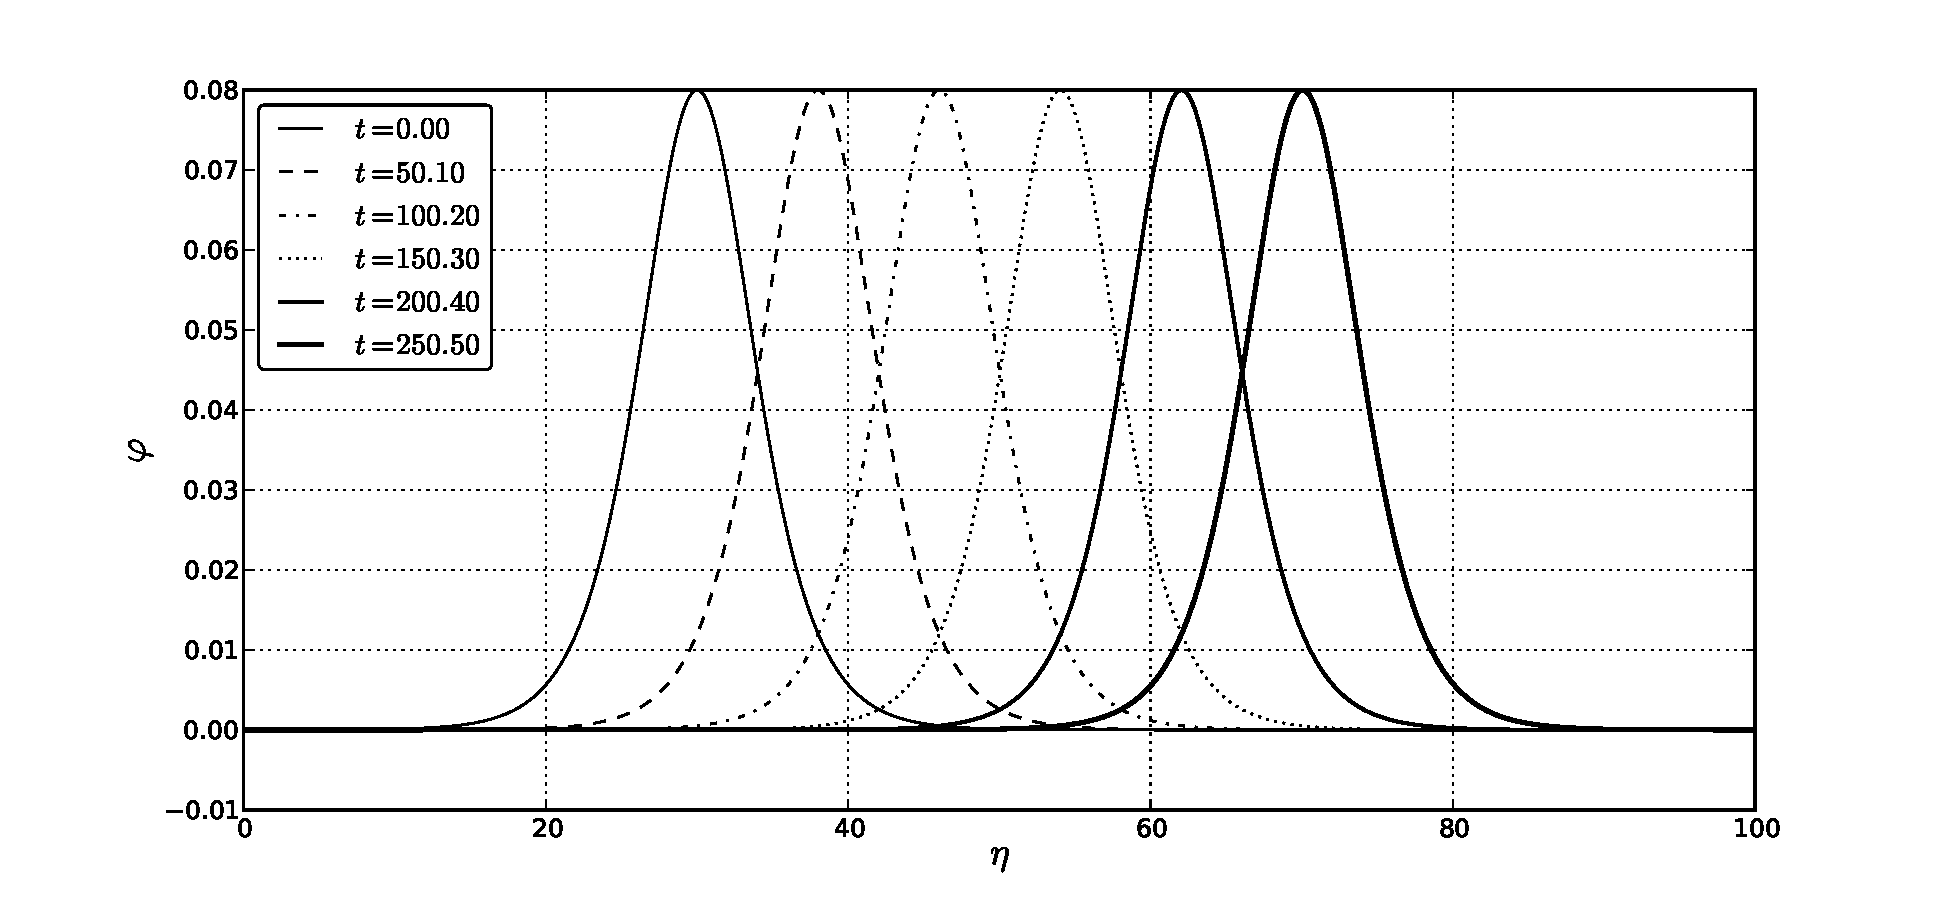
\includegraphics[width=1.0\linewidth]{extract1}}
\caption{Проверка точного решения}
\label{fig11}
\end{figure}

\begin{landscape}
\begin{figure}[H]
\centerline{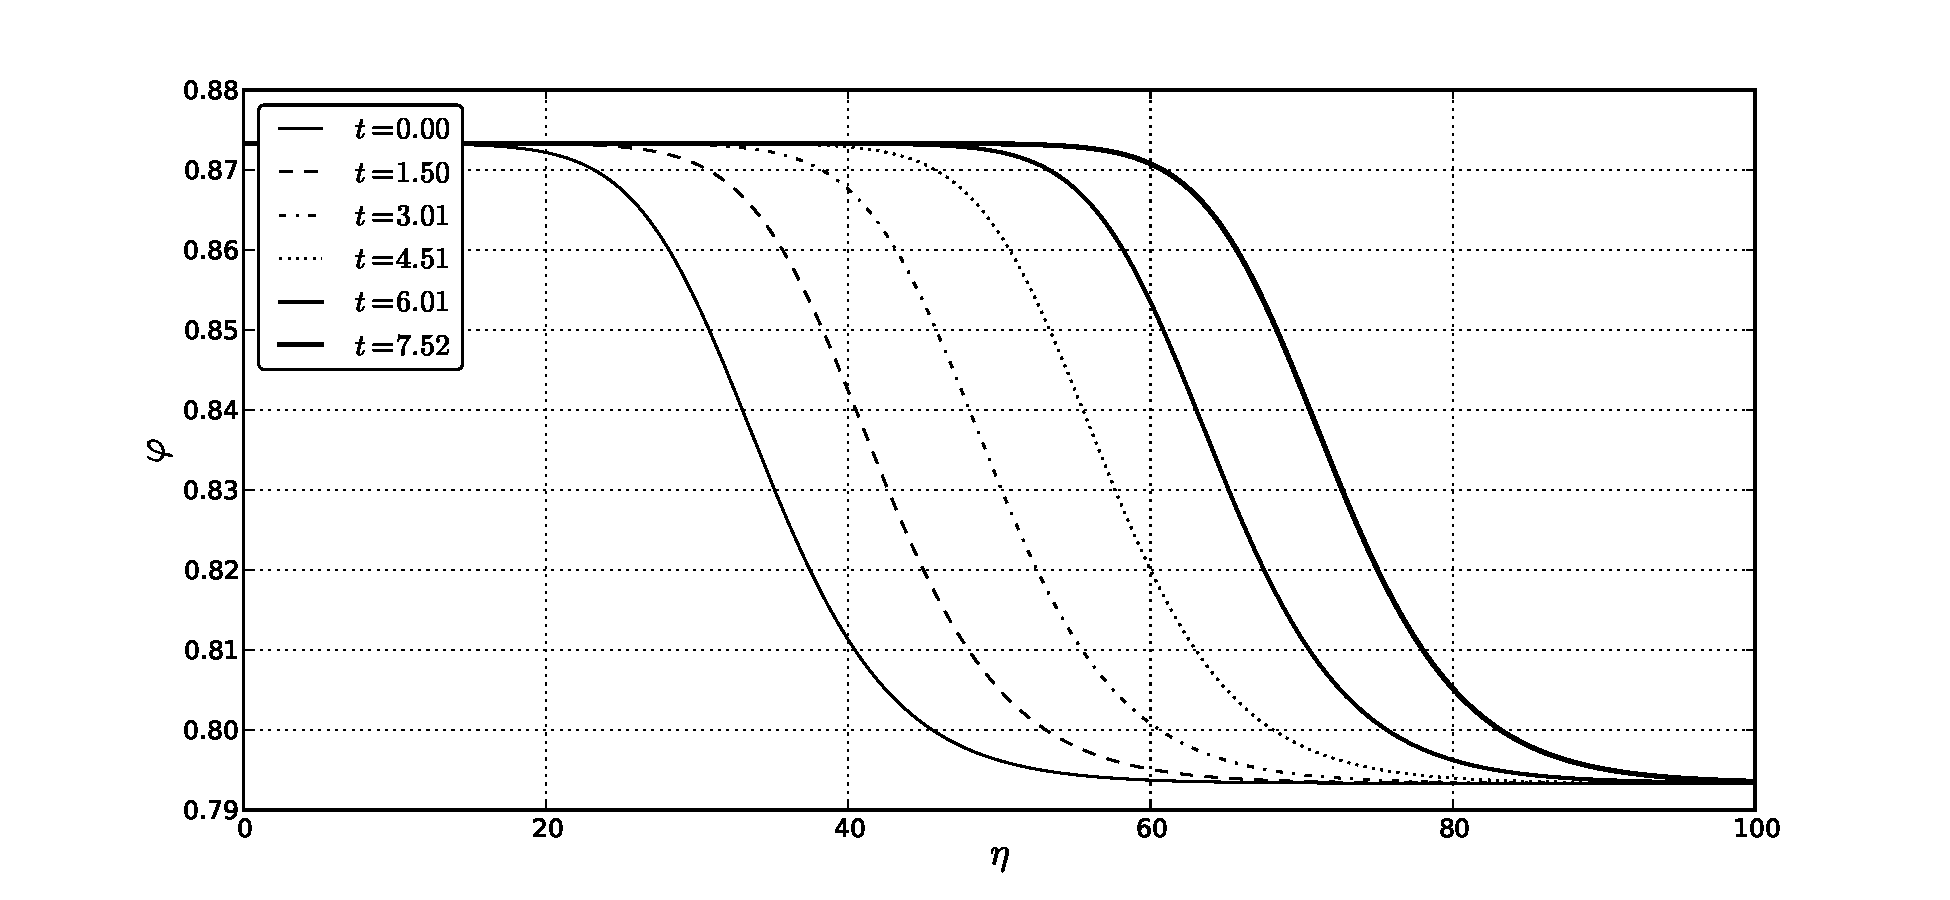
\includegraphics[width=1.0\linewidth]{extract2}}
\caption{
Проверка точного решения $\frac{3}{\sigma_{1}} + \frac{\sigma_{2} \sqrt{6}}{6 \sqrt{\sigma_{1}}} 
 + \frac{k \sqrt{6}}{\sqrt{\sigma_{1}}}\operatorname{tanh}\left(
k x + t \left(- 9 \frac{k}{\sigma_{1}} + \frac{1}{6} k \sigma_{2}^{2} + 2 k^{3}\right)\right)
$}
\label{fig12}
\end{figure}
\end{landscape}

\section{Таблицы}
Таблицы применяют для лучшей наглядности и удобства сравнения показателей. 
Цифровой материал, как правило, оформляют в виде таблиц.

Таблицу следует располагать непосредственно после текста, в котором она упоминается впервые, или на следующей странице.
Наименование таблицы, при его наличии, должно отражать ее содержание, быть точным, кратким. 

На все таблицы должны быть ссылки в тексте. При ссылке следует писать слово «таблица~\ref{tab_weight}» с указанием ее номера.

\begin{table}[H]
\caption{Расчет весомости параметров ПП}
\label{tab_weight}
\centering
    \begin{tabular}{|c|c|c|c|c|c|c|c|c|}
    \hline \multirow{2}{*}{Параметр $x_i$} & \multicolumn{4}{c|}{Параметр $x_j$} & 
        \multicolumn{2}{c|}{Первый шаг} & \multicolumn{2}{c|}{Второй шаг} \\
    \cline{2-9} & $X_1$ & $X_2$ & $X_3$ & $X_4$ & $w_i$ & 
        ${K_\text{в}}_i$ & $w_i$ & ${K_\text{в}}_i$ \\
    \hline $X_1$ & 1 & 1 & 1.5 & 1.5 & 5 & 0.31 & 19 & 0.32 \\
    \hline $X_2$ & 1 & 1 & 1.5 & 1.5 & 5 & 0.31 & 19 & 0.32 \\
    \hline $X_3$ & 0.5 & 0.5 & 1 & 0.5 & 2.5 & 0.16 & 9.25 & 0.16 \\
    \hline $X_4$ & 0.5 & 0.5 & 1.5 & 1 & 3.5 & 0.22 & 12.25 & 0.20 \\
    \hline \multicolumn{5}{|c|}{Итого:} & 16 & 1 & 59.5 & 1 \\
    \hline
    \end{tabular}
\end{table}

Таблицу с большим числом строк допускается переносить на другой лист. При
переносе части таблицы на другой лист слово «Таблица~\ref{Namelists}», ее номер и наименование
указывают один раз слева над первой частью таблицы, а над другими частями также
слева пишут слова "Продолжение таблицы" и указывают номер таблицы.

Допускается нумеровать таблицы в пределах раздела. В этом случае номер таблицы
состоит из номера раздела и порядкового номера таблицы, разделенных точкой.

Таблицы каждого приложения обозначают отдельной нумерацией арабскими цифрами с
добавлением перед цифрой обозначения приложения <<таблица~\ref{Namelists}>>. 

\chapter{Математический текст}

\section{Деление целых чисел}

Следующие предложение~(Childs, 1979), будет использоваться для
доказательств теорем.
\begin{proposition} \emph{(Принцип полной упорядоченности).}
Пусть $k_0$ -- произвольное целое число. Тогда всякое непустое множество
целых чисел $ \geq k_0$, имеет наименьший элемент.
\end{proposition}
\begin{proof}
Докажем, что всякое множество целых чисел $ \geq k_0$, неимеющее
наименьшего элемента, должно быть пустым. Пусть $S$ -- множество
целых чисел $ \geq k_0$  без наименьшего элемента. Предположим
$S$ не содержит целых чисел $ \leq k$. При $k = k_0$ это утверждение
истинно, иначе бы $S$ имела наименьший элемент $k_0$. Пусть это
утверждение верно для $k = n$. Тогда $S$ не содержит элементов
$ \leq k = n+1$, иначе $n+1$ наименьший элемент. Поскольку $n$
произвольно, значит $S$ пустое множество.
\end{proof}

Одно из основных свойств целых чисел -- это свойство \emph{делимости}
или \emph{евклидовости}.
\begin{theorem}\emph{(свойство евклидовости).}
Для любого $a$ и любого $b \neq 0$ существуют единственные (целые)
\emph{частное} $q$ и \emph{остаток} $r$, такие, что
$a=b\cdot q + r, \ 0 \leq r < |b|$
\end{theorem}
\begin{proof}
Рассмотрим множество целых чисел вида $a-kb$, где $k$ пробегает все множество
целых чисел
\begin{eqnarray*}
 \ldots, a -2b, a-b , a, a+b, a+2b,  \ldots
\end{eqnarray*}
Выберем в этой последовательности наименьшее неотрицательное
число и обозначим его $r$, и пусть $q$ обозначает соответствующее
значение $k$. Такое $r$ существует, потому что множество $\{ a-kb\}$
содержит отрицательные и неотрицательные значения, а из принципа полной
упорядоченности следует, что непустое множество неотрицательных целых
чисел содержит наименьший элемент. По определению $r=a - qb$.

Для доказательства единственности допустим, что
\begin{eqnarray*}
a=b\cdot \hat q + \hat r, \ 0 \leq \hat r < |b|
\end{eqnarray*}
и что $\hat r \neq r$. Пусть для определенности $\hat r < r$, так что
$0 < r - \hat r < |b|$, тогда
\begin{eqnarray*}
  r - \hat r = (\hat q - q)b
\end{eqnarray*}
и $b \mid (r - \hat r)$, что противоречит неравенствам
$0 < r - \hat r < |b|$.
\end{proof}

\section{Наибольший общий делитель}

\begin{definition}
Пусть $a$, $b$ одновременно не равны нулю. Целое число $d > 0$
называется \emph{наибольшим общим делителем} $a$ и $b$, если
\begin{enumerate}
  \item $d \mid a$ и $d \mid b$
  \item если $c \mid a$ и $c \mid b$, то $c \mid d$.
\end{enumerate}
\end{definition}
 Наибольший общий делитель $a$ и $b$ будем обозначать $\gcd(a, b)$.
Единственность наибольшего общего делителя следует из свойства~(2)
определения и того, что он положителен.  В самом деле, если
$\hat d$ -- другой наибольший общий делитель, тогда $\hat d \mid d$,
$d \mid \hat d$  и $\hat d = d$, поскольку оба положительны.

\begin{theorem}\emph{(существование $\gcd$).} \label{223}
Если $a$ и $b$ одновременно не равны нулю, то существуют
целые числа $x$ и $y$, такие что $\gcd(a, b) = ax+by$.
\end{theorem}
\begin{proof}
Пусть $d$ -- наименьшее положительное целое число вида $ax+by$.
Согласно принципу полной упорядоченности такое число, например
$d = ax_0+by_0$ существует. Тогда по построению выполняется
свойство~(2) определения наибольшего общего делителя,
если $c \mid a$ и $c \mid b$, то $c \mid (ax_0+by_0) = d$.
Допустим, что свойство~(1) не выполняется, и предположим, для
определенности, что $d$ не делит $b$. Тогда $b = d\cdot q + r$,
$0 < r < d$, и, следовательно, $d > r = b - dq = b - (ax_0+by_0)q=
a(-qx_0)+b(1-qy_0)> 0$, что противоречит минимальности $d$.
\end{proof}

Соотношение $\gcd(a, b) = ax+by$ носит название \emph{соотношения Безу}.
Теорема~(\ref{223}) не утверждает, что $x$ и  $y$ определены
однозначно, она лишь говорит о том, что
наибольший общий делитель может быть выражен в таком виде.

\begin{example}

\begin{tabular}[H]{|c|c|c|c|c|}
\hline
  $a$ & $b$ & $\gcd(a, b)$ & $x$ & $y$  \\ \hline
  36 & 24 & 12 & 1 & -1 \\ \hline
  -36 & 24 & 12 & 3 & 4 \\ \hline
  40 & 24 & 8 & 2 & -3 \\ \hline
  40 & 24 & 8 & 5 & -8 \\ \hline
  36 & 25 & 1 & 16 & -23 \\ \hline
  36 & 25 & 1 & -34 & 49 \\ \hline
\end{tabular}

\end{example}

Пользуясь понятием наибольшего общего делителя, мы можем
охарактеризовать целые решения линейных уравнений, от
двух переменных (\emph{линейных диофантовых уравнений}).
\begin{theorem} Рассмотрим уравнение вида $ax+by = c$,
 в котором $a$ и $b$ не равны нулю одновременно,
 и пусть $d = \gcd(a, b)$. Тогда
\begin{enumerate}
  \item уравнение разрешимо относительно $x$ и $y$ тогда и
    только тогда, когда $d \mid c$,
  \item если $x_0$, $y_0$ -- частное решение, то все решения
    имеют вид $x_0 - n (b/d)$, $y_0 + n (a/d)$ для всех $n$.
\end{enumerate}
\end{theorem}
\begin{proof}
Поскольку $d \mid a$ и $d \mid b$  то $d \mid c$. Следовательно
$c= d \cdot k$ для некоторого целого $k$.  По теореме~(\ref{223})
существуют целые числа $s, t$, такие, что $d = as+bt$.
Умножая это равенство на $k$, получим $c= dk = a(sk) + b(tk)$,
откуда следует, что $x = sk$ и $y = tk$ удовлетворяют
уравнению $ax+by = c$.

Для доказательства второй части, предположим $ax_0+by_0 = c$,
тогда $a(x_0- n (b/d))+ b(y_0+ n (a/d)) = c$ для любого
целого $n$, поскольку $d \mid a$, $d \mid b$, и следовательно
$a n (b/d) = b n (a/d)$.
\end{proof}

\begin{example}
Уравнение $40x+ 24y = 4$ неразрешимо, поскольку $\gcd(40, 24) = 8$ не
делит $4$.

Уравнение $36x+ 25y = c$ разрешимо, поскольку $\gcd(40, 24) = 1$
делит любое число и его решения можно представить ввиде
$x= (16 - 25n)c, y=(-23+36n)c$.
\end{example}

\begin{definition}
Два целых числа $a$ и $b$ называются взаимно простыми, если
$\gcd(a,b)=1$.
\end{definition}
Согласно теореме~(\ref{223}) это равносильно существованию
целых чисел $s, t$, таких, что $as+bt =1$. Справедлива
следующая теорема.

\begin{theorem}
Пусть $a$ и $b$ одновременно не равны нулю,
тогда $a/\gcd(a, b)$ и $b/\gcd(a, b)$ взаимно просты.
\label{225}
\end{theorem}
\begin{proof}
По теореме~(\ref{223}) существуют
целые числа $s, t$, такие, что $\gcd(a, b)=as+bt$. Разделив на $d=\gcd(a, b)$ получим
$1= (a/d)s+(b/d)t$, что влечет за собой $\gcd(a/d, b/d)=1$.
\end{proof}

Эта теорема дает обоснование для введения следующей процедуры $\mathrm{S}$
канонизации~(задача вычисления единственного представ\-ле\-ния для эквивалентных
 объектов) рациональных чисел. Пусть
$$\mathrm{S}\left(\frac{a}{b}\right) = \frac{a/\gcd(a,b)}{b/\gcd(a,b)}$$
тогда, поскольку  $b \neq 0$, то наибольший общий делитель
всегда определен и
$$\frac{a}{b}=
\frac{c}{d} \Rightarrow \mathrm{S}\left(\frac{a}{b}\right)=
\mathrm{S}\left(\frac{c}{d}\right)$$

\section{Алгоритм Евклида}

Основой алгоритма Евклида служит
следующий факт: если $d \mid a$ и $d \mid b$, то $d \mid (a - b \cdot q)$ для
любого целого $q$. В частности, если выбрать в качестве
$d = \gcd(a, b)$ и  $q = a/b$, при $b \neq 0$, получим
$\gcd(a, b) = \gcd(a, a-bq) = \gcd(a, a \mod b)$. Если $b = 0$,
то по определению наибольшего общего делителя имеем
$\gcd(a, 0) = a$. В результате имеем следующий алгоритм:

\begin{Verbatim}[fontsize=\small,numbers=left,firstnumber=last,xleftmargin=7mm]
def Euclid(a, b):
  assert a != 0 or b != 0
  while b != 0:
    a, b = b, a % b
  return a
\end{Verbatim}
Обоснованием окончания алгоритма служит тот факт, что во-время выполнения
из $a \geq b$ следует $a > a \mod b$ по определению остатка от деления.

Для различных приложений очень важно уметь представлять
наибольший общий делитель чисел $a$ и $b$ в виде соотношения
Безу $\gcd(a, b) = ax+by$. Для этого можно воспользоваться
алгоритмом Евклида поскольку остаток от деления, на
каждом шаге алгоритма, можно представить в виде линейной
комбинации делителя и делимого. В качестве иллюстрации
рассмотрим  следующую последовательность
\begin{eqnarray*}
\begin{array}{ll}
a_0 = a, & a_0 = a x_0 + b y_0, \\
a_1 = b, & a_1 = a x_1 + b y_1, \\
a_2 = a_0 - a_1 q_1, & a_2 = a x_2 + b y_2, \\
\ldots & \\
a_i = a_{i-2} - a_{i-1} q_{i-1}, \quad & a_i = a x_i + b y_i, \\
\ldots & \\
a_k = a_{k-2} - a_{k-1} q_{k-1}, & a_k = a x_k + b y_k, \\
0 = a_{k-1} - a_{k} q_{k}, & 0 = a x_{k+1} + b y_{k+1}
\end{array}
\end{eqnarray*}
Очевидно, что $x_0 = 1, y_0 = 0$ и $x_1 = 0, y_1 = 1$. Сравнивая
обе части на $i$-м шаге, имеем
\begin{eqnarray*}
 a x_i + b y_i &=& a_{i-2} - a_{i-1} q_{i-1} = \\
       &=& (a x_{i-2} + b y_{i-2}) - (a x_{i-1} + b y_{i-1}) q_{i-1} = \\
   &=& a (x_{i-2} - x_{i-1} q_{i-1})
     + b (y_{i-2}) - y_{i-1} q_{i-1}).
\end{eqnarray*}
В результате имеем следующий алгоритм называемый
расширенным алгоритмом Евклида:
\begin{Verbatim}[fontsize=\small,frame=leftline]
def EuclidExt(a, b):
  assert a != 0 or b != 0
  a0, a1, b0, b1 = 1, 0, 0, 1
  while b != 0:
    q, r = divmod(a, b)
    a, b = b, r
    a0, a1, b0, b1 = b0, b1, a0 - q*b0, a1 - q*b1
  return (a, a0, a1)
\end{Verbatim}

\section{Непрерывные дроби}
Алгоритм Евклида тесным образом связан с \emph{непрерывными} или
\emph{цепными дробями}. Рассмотрим произвольную рациональную дробь,
записанную в несократимом виде $a_0/a_1$. Применив к паре  $a_0, a_1$
алгоритм Евклида получим
\begin{eqnarray*}
\begin{array}{ll}
  a_0 = a_1\, c_0 + a_2, &  0 < a_2 < a_1, \\
  a_1 = a_2\, c_1 + a_3, &  0 < a_3 < a_2, \\
  \ldots \\
  a_{k-2} = a_{k-1}\, c_{k-2} + a_k, \quad  & 0 < a_{k} < a_{k-1}, \\
  a_{k-1} = a_{k}\, c_{k-1}. &
\end{array}
\end{eqnarray*}
В результате получим следующие каноническое представление для
рациональных дробей; если использовать условие $c_{k-1} > 1$
поскольку $a_{k} < a_{k-1}$
\begin{eqnarray}
 \frac{a_0}{a_1}= c_0 + /c_1, c_2, \ldots, c_n  / = \frac{\displaystyle 1}{\displaystyle c_1
 + \frac{\displaystyle 1}{\displaystyle c_2
 + \frac{\displaystyle 1}{\displaystyle \ddots \qquad
   \frac{\vphantom{\vdots} \displaystyle 1}{\displaystyle c_{n-1}
 + \frac{\displaystyle 1}{\displaystyle c_n}}}}}.
\end{eqnarray}
Числа $c_j$  называют \emph{неполными частными}.
\begin{definition}
Полином, определяемые следующими правилами
\begin{eqnarray*}
 Q_n(c_1, c_2, \ldots, c_n) = \left\{
  \begin{array}{lr}
    1,   & \mbox{при } n = 0 \\
    c_1, & \mbox{при } n = 1 \\
   c_1 \, Q_{n-1}(x_2, \ldots, x_n) + & \\
    \hphantom{+++} + Q_{n-2}(x_3, \ldots, x_n) & \mbox{при } n > 0
  \end{array}
 \right.
\end{eqnarray*}
называются <<континуантами>> или $Q$-многочленами.
\end{definition}
Нам также потребуются числа Фибоначчи определяемые по правилам:
\begin{eqnarray*}
  \mathcal{F}_{n} = \left\{
  \begin{array}{lr}
    1,   & \mbox{при } n = 1 \\
    1, & \mbox{при } n = 2 \\
  \mathcal{F}_{n-1} + \mathcal{F}_{n-2}& \mbox{при } n > 2
  \end{array}
 \right.
\end{eqnarray*}

Следующая теорема нам потребуется при доказательстве теоремы Ламэ.
\begin{theorem} $Q$-многочлены имеют следующие свойства:\\
1.
\begin{eqnarray*}
  /c_1, c_2, \ldots, c_n  / = Q_{n-1}(c_2, \ldots, c_n)/
                           Q_n(c_1, \ldots, c_n), \quad n \geq 1
\end{eqnarray*}
2. Число мономов в $Q$-многочлене равно в точности $\mathcal{F}_{n+1}$
 с коэффициентами равными $1$
\\
3.
\begin{eqnarray*}
\lefteqn{Q_{n}(c_1, \ldots, c_n) Q_n(c_2, \ldots, c_{n+1})-}
\\
& & - Q_{n+1}(c_1, \ldots, c_{n+1}) Q_{n-1}(c_2, \ldots, c_{n})
 = (-1)^n,  \quad n \geq 1
\end{eqnarray*}
 \label{l16}
\end{theorem}
\begin{proof} Все три свойства будут доказаны с использованием
математической индукции.

1. Согласно $/c_1/ = {1}/{ c_1}$, это свойство верно для $n=1$  и предположим
его выполнение для $n=k$. Согласно определению непрерывных дробей
и $Q$-многочленов будем иметь
\begin{eqnarray*}
 /c_1, c_2, \ldots, c_{k+1}/ & =& \frac{1}{c_1 + /c_2, \ldots, c_{k+1}/}
 \\
  &=& \frac{1}{c_1 + Q_{k-1}(c_3, \ldots, c_{k+1})/ Q_k(c_2, \ldots, c_{k+1})}
 \\
 &=& \frac{Q_k(c_2, \ldots, c_{k+1})}
   {c_1\, Q_k(c_2, \ldots, c_{k+1}) + Q_{k-1}(c_3, \ldots, c_{k+1})}
 \\
&=& Q_k(c_2, \ldots, c_{k+1})/Q_{k+1}(c_1, \ldots, c_{k+1}).
\end{eqnarray*}

2. Согласно определению $Q$-многочленов число мономов при $n=1$ равно
$\mathcal{F}_{1} = 1$ и $n=2$ соответственно $\mathcal{F}_{2} = 1$. Докажем,
что из выполнения свойства при $n=k$ следует его истинность при  $n=k+1$.
Согласно определению
\begin{eqnarray*}
 Q_n(c_1,  \ldots, c_{k+1}) =
   c_1 \, Q_{k}(c_2, \ldots, c_n) + Q_{k-1}(c_3, \ldots, c_n)
\end{eqnarray*}
и поскольку полином $Q_{k-1}(c_3, \ldots, c_n)$ не зависит от $c_1$, то
полином $Q_n(c_1,  \ldots, c_{k+1})$ будет иметь коэффициентами при
мономах $1$ и их количество будет равно сумме мономов образующих
его полиномов  $\mathcal{F}_{k} + \mathcal{F}_{k-1} = \mathcal{F}_{k+1}$.


3. При $n=1$ имеем
$c_1 \, c_2 - (c_1 \, c_2 + 1) \cdot 1 = (-1)^1$.
Докажем следование $n=k+1$ из истинности свойства при $n=k$ используя
определение $Q$-многочленов.
\begin{eqnarray*}
\lefteqn{Q_{k+1}(c_1, \ldots, c_{k+1}) Q_{k+1}(c_2, \ldots, c_{k+2})-}
\\
& &-Q_{k+2}(c_1, \ldots, c_{k+2}) Q_{k}(c_2, \ldots, c_{k}) =
\\
\lefteqn{(c_1\, Q_{k}(c_2, \ldots, c_{k+1})
+ Q_{k-1}(c_3, \ldots, c_{k+1})) Q_{k+1}(c_2, \ldots, c_{k+2})-}\\
&&- (c_1\,Q_{k+1}(c_2, \ldots, c_{k+2}) + Q_{k}(c_3, \ldots, c_{k+2}))
Q_{k}(c_2, \ldots, c_{k+1})= \\
\lefteqn{-Q_{k}(c_3, \ldots, c_{k+2}) Q_{k}(c_2, \ldots, c_{k+1}) +}\\
&&+ Q_{k-1}(c_3, \ldots, c_{k+1}) Q_{k+1}(c_2, \ldots, c_{k+2}) = (-1)^{k+1}
\end{eqnarray*}
\end{proof}
Согласно третьему свойству доказанной выше теоремы
$Q_{n}(c_1, \ldots, c_n)$ и $Q_{n-1}(c_2, \ldots, c_n)$ взаимно просты.
Следовательно любая дробь $b/a < 1$ может быть представлена в виде
\begin{eqnarray}
\frac{b}{a} = \frac{Q_{n-1}(c_2, \ldots, c_n)\, \gcd(a, b)}
                   {Q_{n}(c_1, \ldots, c_n)\, \gcd(a, b)}
 \label{l17}
\end{eqnarray}
Теперь возможно рассмотрение поведение алгоритма Евклида в
<<наихудшем случае>>, другими словами дать верхнюю границу числа
шагов деления.

\section{Теорема Ламэ}

\begin{theorem}\emph{(G. Lam\'e 1845.)}
Пусть при $r \geq 1$ целые числа $a$ и $b$, $0 < b < a$, такие, что
алгоритм Евклида, примененный к $a$ и $b$, требует в точности
$r$ шагов деления, и такие, что $a$ есть наименьшее из возможных
чисел, удовлетворяющих этим условиям. Тогда $a =\mathcal{F}_{r+2}$
и $b =\mathcal{F}_{r+1}$.
\label{lam}
\end{theorem}
\begin{proof} В силу~(\ref{l17}) мы должны иметь для
$$b =Q_{r-1}(c_2, \ldots, c_{r})\, \gcd(a, b)$$ и
$$a =Q_{r}(c_1, \ldots, c_{r})\, \gcd(a, b)$$. Поскольку согласно
второму свойству теоремы~\ref{l16} $Q$-многочлен состоит из
мономов c коэффициентами равными $1$,
минимальное значение достигается тогда, когда
$c_1=1, \ldots, c_{r-1}=1, \, c_{r}=2, \, \gcd(a, b) =1$.
Используя определение $Q$-многочленов в результате получим
для $r=1$ \ $c_{1}=2$, $a =\mathcal{F}_{3}$ и $b =\mathcal{F}_{2}$,
и следовательно для $r=k$ \ $a =\mathcal{F}_{k+2}$ и $b =\mathcal{F}_{k+1}$.
\end{proof}
Эта теорема явилась первым практическим применением последовательности
Фибоначчи, с тех пор было дано много других применений чисел
Фибоначчи к алгоритмам и к исследованию алгоритмов.

Для рассмотрения следствия этой теоремы нам понадобится
понятие <<золотого сечения>>. Пусть $a > b > 0$ две величины
связанные соотношением
\begin{eqnarray*}
 \phi = \frac{a+b}{a} = 1 + \frac{b}{a} = \frac{a}{b}
\end{eqnarray*}
откуда решая квадратное уравнение,
выбирая корень для
которого $a > b$, получим $\phi = (\sqrt{5} + 1)/2 = 1.61803\, 39887 \ldots$.
Поскольку
\begin{eqnarray*}
 \lim_{n \to +\infty}\frac{\mathcal{F}_{n+1}}{\mathcal{F}_{n}} =
 \lim_{n \to +\infty}\frac{\mathcal{F}_{n} + \mathcal{F}_{n-1}}{\mathcal{F}_{n}}=
 1+ \frac{1}{\lim_{n \to +\infty}\frac{\mathcal{F}_{n}}{\mathcal{F}_{n-1}}}= \phi
\end{eqnarray*}
будем иметь следующую формулу для чисел Фибоначчи
$ \displaystyle
\mathcal{F}_{n}  \approx \left\lceil \frac{\phi^n}{\sqrt{5}}\right\rceil
$
\begin{corollary}
Если $0 < b < a$, то число шагов деления,
необходимых алгоритма Евклида для обработки
$a$, $b$ не превышает
$\left\lceil \log_\phi(\sqrt{5}\, b)) \right\rceil - 2$
\label{lame}
\end{corollary}
\begin{proof}
Согласно теореме \ref{lam} максимальное число шагов  $r$ имеет
место в случае, когда $a =\mathcal{F}_{r+2}$ и $b =\mathcal{F}_{r+1}$.
В результате по формуле для чисел Фибоначчи будем иметь
\begin{eqnarray*}
b < \left\lceil \frac{\phi^{r+2}}{\sqrt{5}}\right\rceil
\end{eqnarray*}
или $r < \left\lceil \log_\phi(\sqrt{5}\, b) \right\rceil - 2$.
\end{proof}
Заметим $\log_\phi(\sqrt{5}\, b) \approx 4.785 \, \log_{10} \, b + 1.672$
и возможна формулировка этого следствия использующая число десятичных цифр.

Как правило если существует одна оценка, то существуют много других
не совпадающих с первой. Мы приведем несколько примеров:
\begin{theorem}~\cite{DBLP:journals/ipl/CollinsM77}
Если $0 < b < a$, то число шагов деления,
необходимых алгоритма Евклида для обработки
$a$, $b$ не превышает
$(\log_\phi \, 2)\cdot \mathcal{F}_\beta(b)  + 2$.
\end{theorem}
\begin{theorem}\emph{(С.А. Абрамов 1979.)}
Пусть $a,\, b$ -- целые положительные числа, то число шагов деления,
необходимых алгоритму Евклида для обработки
$a$ и $b$ не превосходит
$\left\lfloor \log_2 \, \max(a, b) \right\rfloor + 1$.
\end{theorem}

\begin{theorem}\emph{(E. Ces\'aro 1881.)}
Если $a < b$ -- случайно выбираемые целые числа,
то вероятность того, что $\gcd(a, b) = 1$, равна
$6/\pi^2$.
\end{theorem}
Согласно этой теореме в $6/\pi^2 \approx 61\%$ случаях
наибольшим общем делителем является $1$, поэтому
для алгоритма Евклида актуальным остается
оценка временной сложности в среднем.

\chapter{Диаграммы UML}

В соответствии с рисунком~\ref{sms} представлена диаграмма состояний
построенная с помощью следующего кода на сайте
\url{http://www.plantuml.com/plantuml/}.
\begin{Verbatim}[fontsize=\small,frame=leftline]
[*] --> outbox
outbox -> отправка : С частотой 2 раза в сек.
отправка --> bounced : Известная ошибка,\nтребующая повторной\nотправки
отправка --> sent : Отправка без ошибок
отправка --> error : Неизвестная ошибка\nпри отправке
отправка --> overlimit : Превышен лимит\nотправок
overlimit --> [*]  
sent --> [*]
error --> [*]
bounced --> outbox : После выдержки 1 минимальное
\end{Verbatim}

\begin{figure}[H]
\centerline{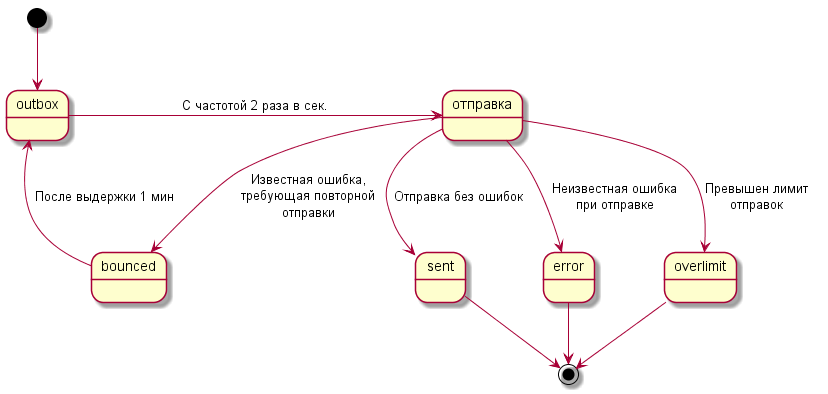
\includegraphics[width=1.0\linewidth]{sms.png}}
\caption{Отправка sms через интернет ресурс}
\label{sms}
\end{figure}

Примеры других типов диаграмм можно взять
по адресу \url{http://plantuml.sourceforge.net/}.
Например следующий ниже код соответствует диаграмме, представленной на рисунке ~\ref{class}.
\begin{Verbatim}[fontsize=\small,frame=leftline]
class BaseClass

namespace net.dummy #DDDDDD
    .BaseClass <|-- Person
    Meeting o-- Person
    
    .BaseClass <|- Meeting

end namespace

namespace net.foo {
  net.dummy.Person  <|- Person
  .BaseClass <|-- Person

  net.dummy.Meeting o-- Person
}

BaseClass <|-- net.unused.Person
\end{Verbatim}

\begin{figure}[H]
\centerline{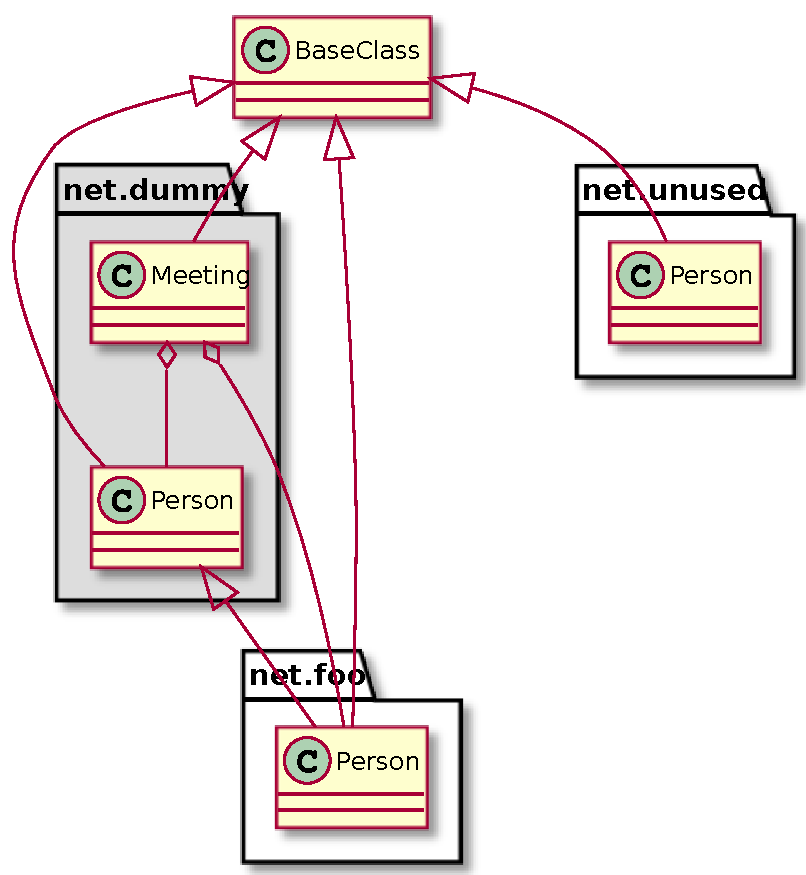
\includegraphics[width=0.5\linewidth]{class}}
\caption{Пример диаграммы классов}
\label{class}
\end{figure}
Для улучшения качества рисунка, нужно его
сохранить в формате SVG, а затем перевести в формат PDF
с помощью бесплатного редактора векторной графики \url{http://inkscape.org/}.

\conclusions

Заключение, как правило, должно содержать: 
\begin{itemize}
\item основные результаты работы и краткие выводы по ним;
\item оценку полноты решений поставленных задач;
\item рекомендации по использованию результатов работы;
\item результаты оценки эффективности предложенных решений и сопоставление с лучшими достижениями в данной области.
\end{itemize}

% Оформляем библиографию в соответствии с ГОСТ 7.0.5
% \bibliographystyle{ugost2008}
% если хотим включить все источники из библиографии даже не имеющие ссылки из текта
% \nocite{*}
% файл с библиографией
% \bibliography{biblio.bib}

\newpage
\begin{thebibliography}{99}
\bibitem{bib1} Что такое NoSQL? [Электронный ресурс]: [сайт]. - URL: \url{https://aws.amazon.com/ru/nosql} (дата обращения: 13.03.2019). - Загл. с экрана. - Яз.рус.

\bibitem{bib2} Балдин, К. В. Информационные системы в экономике [Электронный ресурс]: учебник / Балдин К. В. - Москва : Дашков и К, 2015. - Загл. с экрана.

\bibitem{bib3} Гагарина, Л. Г. Разработка и эксплуатация автоматизированных информационных систем : Учебное пособие / Л. Г.Гагарина. - 2-е изд., перераб. и доп.  М.: Издательский Дом <<ФОРУМ>> ; Москва : ООО <<Научноиздательский центр ИНФРА-М>>, 2017. - 384 с.

\bibitem{bib4} Заботина, Н. Н. Проектирование информационных систем: Учебное пособие / Наталья Николаевна Заботина.  М.: ООО ѕНаучно-издательский центр ИНФРА-Мї, 2013. - 331 с.

\bibitem{bib5} Шкундин, С. З. Теория информационных процессов и систем [Электронный ресурс] / С. З. Шкундин, В. Ш. Берикашвили. - Москва : Горная книга, 2012. - 475 с.: ил. - Библиогр. : - 471 c.

\bibitem{bib6} Реляционные базы данных: достоинства и недостатки [Электронный
ресурс]: [сайт]. - URL: \url{https://sites.google.com/site/gosyvmkss12/bazydannyh/07-relacionnye-bazy-dannyh-dostoinstva-i-nedostatki} (дата обращения: 01.02.2019). - Загл. с экрана. - Яз.рус.

\bibitem{bib7} Головицына, М. В. Информационные технологии в экономике [Электронный ресурс]: учебное пособие / Головицына М. В.  М.: ИнтернетУниверситет Информационных Технологий (ИНТУИТ), 2016. - 405 с.

\bibitem{bib8} SQL и NoSQL : основные модели баз данных [Электронный ресурс]:
[сайт].  URL: \url{https://tproger.ru/translations/sql-nosql-database-models/}
(дата обращения: 11.03.2019). - Загл. с экрана. - Яз.рус.

\bibitem{bib9} СУБД NOSQL  сильные и слабые стороны [Электронный ресурс]: [сайт].
- URL: \url{http://www.jetinfo.ru/stati/silnye-i-slabye-storony-nosql} (дата обращения:13.03.2019). - Загл. с экрана. - Яз.рус.

\bibitem{bib10} Фаулер, М. NoSQL. Новая методология разработки нереляционных баз
данных. / М. Фаулер, П. Садаладж.  М.: ДМК-Пресс, 2013. - 158 c.

\bibitem{bib11} Memcached - a distributed memory object caching system [Электронный ресурс]: [сайт]. - URL: 
\url{http://memcached.org/} (дата обращения: 14.01.2019). - Загл. с экрана. - Яз.рус.

\bibitem{bib12} OrientDB [Электронный ресурс]: [сайт]. - URL: \url{https://orientdb.com/} (дата обращения:13.12.2018). - Загл. с экрана. - Яз.рус.

\bibitem{bib13} DB-Engines Ranking [Электронный ресурс]: [сайт]. - 
URL: \url{http://dbengines.com/en/ranking} (дата обращения: 13.12.2018). - Загл. с экрана. Яз.рус.

\bibitem{bib14} NOSQL Databases [Электронный ресурс]: [сайт]. - URL: 
\url{http://www.sqltutorial.ru/ru/book_graph_databases.html} (дата обращения:17.01.2019). Загл. с экрана. - Яз.рус.

\bibitem{bib15} Бенкер, К. MongoDB в действии / К. Бенкер.  М.: ДМК пресс, 2016. 246 с.


\bibitem{bib16} Карвин, Б. Программирование бах данных SQL. Типичные ошибки и их
устранение / Б. Карвин.  М.: Рид Групп, 2011. - 110 с.

\bibitem{bib17} Агальцов, В. П. Базы данных: учебное пособие для вузов: В 2 книгах
Книга 2 : Распределенные и удаленные базы данных / В. П. Агальцов. 1.  М.: Издательский Дом ѕФОРУМї, 2017. - 271 с.

\bibitem{bib18} SQL, NOSQL И ДРУГИЕ МОДЕЛИ БАЗ ДАННЫХ [Электронный ресурс]: [сайт]. - URL:
\url{https://www.8host.com/blog/sql-nosql-i-drugie-modelibaz-dannyx} - Загл. с экрана. - Яз.рус.

\bibitem{bib19} SQL и NoSQL: разбираемся в основных моделях баз данных [Электронный ресурс]: [сайт]. - 
URL: \url{https://tproger.ru/translations/sql-nosqldatabase-models} (дата обращения: 13.03.2019). - Загл. с экрана. - Яз.рус.

\bibitem{bib20} Кузнецов, С. Базы данных. Модели и языки / С. Кузнецов.  М.: БиномПресс, 2008. - 560 с.
\end{thebibliography}


\Appendix % Приложения

\chapter{Исходные коды реализации алгоритма Евклида}
\begin{Verbatim}[fontsize=\small,numbers=left,firstnumber=1,stepnumber=1]
# -*- coding: utf-8 -*-

"""
Реализация алгоритмов наибольшего общего делителя
"""

def Euclid(a, b):
  assert a != 0 or b != 0
  while b != 0:
    a, b = b, a % b
  return a

def EuclidExt(a, b):
  assert a != 0 or b != 0
  a0, a1, b0, b1 = 1, 0, 0, 1
  while b != 0:
    q, r = divmod(a, b)
    a, b = b, r
    a0, a1, b0, b1 = b0, b1, a0 - q*b0, a1 - q*b1
  return (a, a0, a1)

if __name__ == '__main__':
  a, b = 1231231232*123, 123681726382*123
  print Euclid(a, b)
  g, x, y = EuclidExt(a, b)
  print a*x + b*y, "= %d*%d + %d*%d" % (a, x, b, y)
\end{Verbatim}

\chapter{Очень длинное название второго приложения \label{AppendixB}}


\fontsize{10pt}{10pt}\selectfont
\begin{longtable}[c]{|l|c|l|l|}
\caption{Описание входных файлов модели}\label{Namelists}
\\ \hline
 Параметр & Умолч. & Тип & Описание               \\ \hline
 \endfirsthead   \hline
 \multicolumn{4}{|c|}{Продолжение таблицы~\ref{Namelists}}        \\ \hline
 Параметр & Умолч. & Тип & Описание               \\ \hline
 \endhead        \hline
 \endfoot        \hline
 \multicolumn{4}{|c|}{Параметров \&INP}        \\ \hline 
 kick & 1 & int & 0: инициализация без шума ($p_s = const$) \\
      &   &     & 1: генерация белого шума                  \\
      &   &     & 2: генерация белого шума симметрично относительно \\
  & & & экватора    \\
 mars & 0 & int & 1: инициализация модели для планеты Марс     \\
 kick & 1 & int & 0: инициализация без шума ($p_s = const$) \\
      &   &     & 1: генерация белого шума                  \\
      &   &     & 2: генерация белого шума симметрично относительно \\
  & & & экватора    \\
 mars & 0 & int & 1: инициализация модели для планеты Марс     \\
kick & 1 & int & 0: инициализация без шума ($p_s = const$) \\
      &   &     & 1: генерация белого шума                  \\
      &   &     & 2: генерация белого шума симметрично относительно \\
  & & & экватора    \\
 mars & 0 & int & 1: инициализация модели для планеты Марс     \\
kick & 1 & int & 0: инициализация без шума ($p_s = const$) \\
      &   &     & 1: генерация белого шума                  \\
      &   &     & 2: генерация белого шума симметрично относительно \\
  & & & экватора    \\
 mars & 0 & int & 1: инициализация модели для планеты Марс     \\
kick & 1 & int & 0: инициализация без шума ($p_s = const$) \\
      &   &     & 1: генерация белого шума                  \\
      &   &     & 2: генерация белого шума симметрично относительно \\
  & & & экватора    \\
 mars & 0 & int & 1: инициализация модели для планеты Марс     \\
kick & 1 & int & 0: инициализация без шума ($p_s = const$) \\
      &   &     & 1: генерация белого шума                  \\
      &   &     & 2: генерация белого шума симметрично относительно \\
  & & & экватора    \\
 mars & 0 & int & 1: инициализация модели для планеты Марс     \\
kick & 1 & int & 0: инициализация без шума ($p_s = const$) \\
      &   &     & 1: генерация белого шума                  \\
      &   &     & 2: генерация белого шума симметрично относительно \\
  & & & экватора    \\
 mars & 0 & int & 1: инициализация модели для планеты Марс     \\
kick & 1 & int & 0: инициализация без шума ($p_s = const$) \\
      &   &     & 1: генерация белого шума                  \\
      &   &     & 2: генерация белого шума симметрично относительно \\
  & & & экватора    \\
 mars & 0 & int & 1: инициализация модели для планеты Марс     \\
kick & 1 & int & 0: инициализация без шума ($p_s = const$) \\
      &   &     & 1: генерация белого шума                  \\
      &   &     & 2: генерация белого шума симметрично относительно \\
  & & & экватора    \\
 mars & 0 & int & 1: инициализация модели для планеты Марс     \\
kick & 1 & int & 0: инициализация без шума ($p_s = const$) \\
      &   &     & 1: генерация белого шума                  \\
      &   &     & 2: генерация белого шума симметрично относительно \\
  & & & экватора    \\
 mars & 0 & int & 1: инициализация модели для планеты Марс     \\
kick & 1 & int & 0: инициализация без шума ($p_s = const$) \\
      &   &     & 1: генерация белого шума                  \\
      &   &     & 2: генерация белого шума симметрично относительно \\
  & & & экватора    \\
 mars & 0 & int & 1: инициализация модели для планеты Марс     \\
kick & 1 & int & 0: инициализация без шума ($p_s = const$) \\
      &   &     & 1: генерация белого шума                  \\
      &   &     & 2: генерация белого шума симметрично относительно \\
  & & & экватора    \\
 mars & 0 & int & 1: инициализация модели для планеты Марс     \\
kick & 1 & int & 0: инициализация без шума ($p_s = const$) \\
      &   &     & 1: генерация белого шума                  \\
      &   &     & 2: генерация белого шума симметрично относительно \\
  & & & экватора    \\
 mars & 0 & int & 1: инициализация модели для планеты Марс     \\
kick & 1 & int & 0: инициализация без шума ($p_s = const$) \\
      &   &     & 1: генерация белого шума                  \\
      &   &     & 2: генерация белого шума симметрично относительно \\
  & & & экватора    \\
 mars & 0 & int & 1: инициализация модели для планеты Марс     \\
kick & 1 & int & 0: инициализация без шума ($p_s = const$) \\
      &   &     & 1: генерация белого шума                  \\
      &   &     & 2: генерация белого шума симметрично относительно \\
  & & & экватора    \\
 mars & 0 & int & 1: инициализация модели для планеты Марс     \\
 \hline
  %& & & $\:$ \\ 
 \multicolumn{4}{|l|}{\&SURFPAR}        \\ \hline
kick & 1 & int & 0: инициализация без шума ($p_s = const$) \\
      &   &     & 1: генерация белого шума                  \\
      &   &     & 2: генерация белого шума симметрично относительно \\
  & & & экватора    \\
 mars & 0 & int & 1: инициализация модели для планеты Марс     \\
kick & 1 & int & 0: инициализация без шума ($p_s = const$) \\
      &   &     & 1: генерация белого шума                  \\
      &   &     & 2: генерация белого шума симметрично относительно \\
  & & & экватора    \\
 mars & 0 & int & 1: инициализация модели для планеты Марс     \\
kick & 1 & int & 0: инициализация без шума ($p_s = const$) \\
      &   &     & 1: генерация белого шума                  \\
      &   &     & 2: генерация белого шума симметрично относительно \\
  & & & экватора    \\
 mars & 0 & int & 1: инициализация модели для планеты Марс     \\
kick & 1 & int & 0: инициализация без шума ($p_s = const$) \\
      &   &     & 1: генерация белого шума                  \\
      &   &     & 2: генерация белого шума симметрично относительно \\
  & & & экватора    \\
 mars & 0 & int & 1: инициализация модели для планеты Марс     \\
kick & 1 & int & 0: инициализация без шума ($p_s = const$) \\
      &   &     & 1: генерация белого шума                  \\
      &   &     & 2: генерация белого шума симметрично относительно \\
  & & & экватора    \\
 mars & 0 & int & 1: инициализация модели для планеты Марс     \\
kick & 1 & int & 0: инициализация без шума ($p_s = const$) \\
      &   &     & 1: генерация белого шума                  \\
      &   &     & 2: генерация белого шума симметрично относительно \\
  & & & экватора    \\
 mars & 0 & int & 1: инициализация модели для планеты Марс     \\
kick & 1 & int & 0: инициализация без шума ($p_s = const$) \\
      &   &     & 1: генерация белого шума                  \\
      &   &     & 2: генерация белого шума симметрично относительно \\
  & & & экватора    \\
 mars & 0 & int & 1: инициализация модели для планеты Марс     \\
kick & 1 & int & 0: инициализация без шума ($p_s = const$) \\
      &   &     & 1: генерация белого шума                  \\
      &   &     & 2: генерация белого шума симметрично относительно \\
  & & & экватора    \\
 mars & 0 & int & 1: инициализация модели для планеты Марс     \\
kick & 1 & int & 0: инициализация без шума ($p_s = const$) \\
      &   &     & 1: генерация белого шума                  \\
      &   &     & 2: генерация белого шума симметрично относительно \\
  & & & экватора    \\
 mars & 0 & int & 1: инициализация модели для планеты Марс     \\ 
 \hline 
\end{longtable}

\end{document}
